\documentclass[oneside, 11pt]{article}

\usepackage[T1]{fontenc}
\usepackage[utf8]{inputenc}
\usepackage[dutch]{babel}

\usepackage{fouriernc}
\usepackage[detect-all, load-configurations=binary,
            separate-uncertainty=true, per-mode=symbol,
            retain-explicit-plus, range-phrase={ tot }]{siunitx}

\usepackage{setspace}
\setstretch{1.2}

\setlength{\parskip}{\smallskipamount}
\setlength{\parindent}{0pt}

\usepackage{geometry}
\geometry{marginparwidth=0.5cm, verbose, a4paper, tmargin=3cm, bmargin=3cm, lmargin=2cm, rmargin=2cm}

\usepackage{float}

\usepackage[fleqn]{amsmath}
\numberwithin{equation}{section}
\numberwithin{figure}{section}

\usepackage{graphicx}
\graphicspath{{Figures/}}
\usepackage{subfig}

\usepackage{tikz}
\usetikzlibrary{plotmarks}

\usepackage{fancyhdr}
\pagestyle{fancy}
\fancyhf{}
\rhead{\thepage}
\renewcommand{\footrulewidth}{0pt}
\renewcommand{\headrulewidth}{0pt}

\usepackage{relsize}
\usepackage{xspace}
\usepackage{url}

\newcommand{\figref}[1]{Figuur~\ref{#1}}

\newcommand{\hisparc}{\textsmaller{HiSPARC}\xspace}
\newcommand{\kascade}{\textsmaller{KASCADE}\xspace}
\newcommand{\sapphire}{\textsmaller{SAPPHiRE}\xspace}
\newcommand{\jsparc}{\textsmaller{jSparc}\xspace}
\newcommand{\hdf}{\textsmaller{HDF5}\xspace}
\newcommand{\aires}{\textsmaller{AIRES}\xspace}
\newcommand{\csv}{\textsmaller{CSV}\xspace}
\newcommand{\python}{\textsmaller{PYTHON}\xspace}
\newcommand{\corsika}{\textsmaller{CORSIKA}\xspace}
\newcommand{\labview}{\textsmaller{LabVIEW}\xspace}
\newcommand{\daq}{\textsmaller{DAQ}\xspace}
\newcommand{\adc}{\textsmaller{ADC}\xspace}
\newcommand{\adcs}{\textsmaller{ADC}s\xspace}
\newcommand{\Adcs}{A\textsmaller{DC}s\xspace}
\newcommand{\hi}{\textsc{h i}\xspace}
\newcommand{\hii}{\textsc{h ii}\xspace}
\newcommand{\mip}{\textsmaller{MIP}\xspace}
\newcommand{\hisparcii}{\textsmaller{HiSPARC II}\xspace}
\newcommand{\hisparciii}{\textsmaller{HiSPARC III}\xspace}
\newcommand{\pmt}{\textsmaller{PMT}\xspace}
\newcommand{\pmts}{\textsmaller{PMT}s\xspace}

\DeclareSIUnit{\electronvolt}{\ensuremath{\mathrm{e\!\!\:V}}}

\DeclareSIUnit{\unitsigma}{\ensuremath{\sigma}}
\DeclareSIUnit{\mip}{\textsmaller{MIP}}
\DeclareSIUnit{\adc}{\textsmaller{ADC}}

\DeclareSIUnit{\gauss}{G}
\DeclareSIUnit{\parsec}{pc}
\DeclareSIUnit{\year}{yr}



\title{Pulshoogte en pulsintegraal}
\author{N.G. Schultheiss}
\docwerkblad{2}{PH}
\version{1.0}

\begin{document}

\maketitle

\section{Inleiding}

Elke detector van een \hisparc-station is uitgerust met een
foto-versterker buis (PhotoMultiplier Tube: \pmt). Als er geen deeltjes
door de detector schieten, treedt er geen fluorescentie in de detector
op en ontstaat er geen licht. In dit geval geeft de PMT-buis een
elektrisch signaal van \SI{0}{\milli\volt} aan de \hisparc unit. Als er
wel deeltjes door de detector schieten, treedt er fluorescentie in de
detector op en ontstaat er licht. Dan geeft de PMT-buis een elektrisch
signaal af waarvan het aantal mV afhangt van het aantal deeltjes dat
door de detector is gegaan. In de \hisparc unit wordt het analoge
signaal door middel van een Analoog Digitaal Converter (\adc) omgezet in
een digitaal signaal. De grootte van dit signaal wordt uitgedrukt in
\adcs, de \adc count (een getal zonder eenheid).

Als er een detectorsignaal gemeten wordt, wordt een reeks van deze \adcs
in de \hisparc unit opgeslagen. Als er tegelijkertijd een tweede reeks,
van een andere detector, wordt opgeslagen, worden alle reeksen \adcs van
de \hisparc unit naar de \hisparc server gezonden. Met dergelijke reeks
kan een diagram van het verloop van het signaal tegen de tijd worden
gemaakt. In deze diagrammen zijn van het negatieve maximale signaal de
pulshoogte en het oppervlak, de pulsintegraal, te bepalen. Gedurende de
dag worden alle pulshoogten en pulsintegralen van een station verzameld.
Pulshoogte en pulsintegraal histogrammen zijn op te vragen op:
\url{https://data.hisparc.nl/} door op de stationsnaam te klikken.
Rechtsboven beide histogrammen is een link waarmee de gegevens in een
spreadsheet, zoals Excel, te laden zijn.


\section{De pulsvorm}


\subsection{Pulsen ophalen uit de \hisparc data opslag}

\begin{figure}[ht]
    \centering
    \subfloat{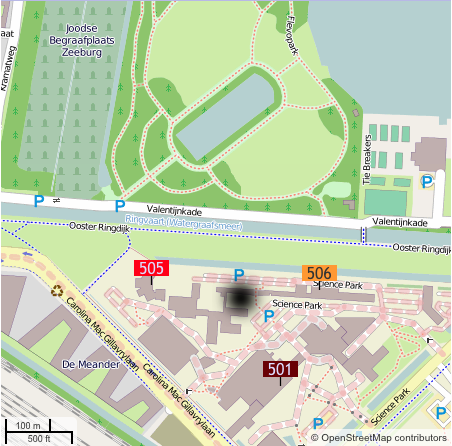
\includegraphics[scale=0.33]{kaart}}
    \subfloat{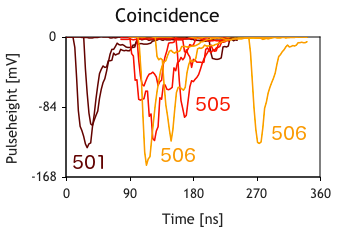
\includegraphics[scale=0.65]{Coincidence}}
    \caption{De plattegrond met de locaties van de meetstations
             en de gemeten pulsen per station.}
    \label{fig:coincidence}
\end{figure}

In de praktijk kunnen we een set pulsen voor een willekeurige
gebeurtenis ophalen met \jsparc%
\footnote{Het interactieve practicum \jsparc kan in de les na aanvraag
van een sessie worden gebruikt, het is ook mogelijk om een willekeurige
set pulsen op te halen op:
\url{https://data.hisparc.nl/media/jsparc/jsparc.html}.%
}. In deze module gaan we uit van de set pulsen die met de stations
uit \figref{fig:coincidence} zijn gemeten.

Op de kaart zijn drie meetstations te zien, een bruin, een rood en een
oranje station%
\footnote{De kleuren van de stations volgen de definitie van de
kleurcode van weerstandjes: bruin: 1, rood: 2, oranje: 3, geel: 4,
groen: 5, blauw: 6, violet: 7, etc. %
}. We zien dat alle stations meerdere pulsen hebben gegeven, dit komt
omdat een station uit meerdere detectoren bestaat. De hoogtes van de
pulsen zijn vergelijkbaar, bijgevolg is het midden van de air-shower
(zwarte vlek in \figref{fig:coincidence}) even ver van alle stations.


\subsection{Eenvoudige pulsvormen}

Het is mogelijk om de diagrammen per detector van een enkel station
te bekijken. In \figref{fig:Eenvoudige-pulsen} zijn de signalen
van vier detectoren van Station 506 te zien. De zwarte puls van detector
1 heeft een vrij steile voorflank. Het verloop van de achterflank
lijkt een halfwaardetijd te hebben (deze loopt exponentieel op). Bij
de blauwe grafiek van detector 4 is iets soortgelijks aan de hand.
Een deeltje lijkt dus herkend te worden aan een steile dalende flank
die wordt gevolgd door een exponentieel oplopende achterflank.

\begin{figure}[ht]
    \centering
    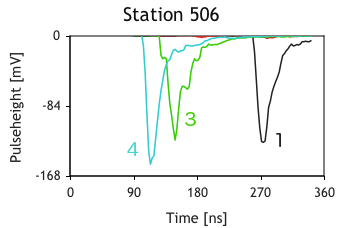
\includegraphics[scale=0.65]{Traces506}
    \caption{Eenvoudige pulsen}
    \label{fig:Eenvoudige-pulsen}
\end{figure}


\begin{minipage}[t]{1\columnwidth}%

\paragraph{Opdracht 1:}

De groene grafiek van detector 3 in \figref{fig:Eenvoudige-pulsen}
heeft een minder vloeiend verloop. Stel een hypothese op waarmee dit
minder vloeiende verloop kan worden verklaard.

\begin{center}
    \rule{\textwidth}{0.3mm}\\
    \rule{\textwidth}{0.3mm}\\
    \rule{\textwidth}{0.3mm}\\
    \rule{\textwidth}{0.3mm}\\
\end{center}
\end{minipage}

\bigskip{}


Meestal zien de grafieken er niet zo mooi uit als in
\figref{fig:Eenvoudige-pulsen}. In \figref{fig:Iets-complexere-pulsen}
zijn andere pulsen van detector 1 en 4 van Station 501 te zien
(respectievelijk zwart en blauw).

\begin{figure}[ht]
    \centering
    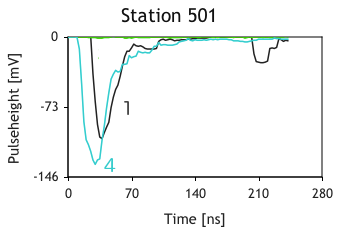
\includegraphics[scale=0.65]{Traces501}
    \caption{Iets complexere pulsen}
    \label{fig:Iets-complexere-pulsen}
\end{figure}


\begin{minipage}[t]{1\columnwidth}%

\paragraph{Opdracht 2:}

Geef een verklaring voor het verloop van de grafiek van detector
1 in \figref{fig:Iets-complexere-pulsen}.

\begin{center}
    \rule{\textwidth}{0.3mm}\\
    \rule{\textwidth}{0.3mm}\\
    \rule{\textwidth}{0.3mm}\\
    \rule{\textwidth}{0.3mm}\\
\end{center}
\end{minipage}

\bigskip{}


\begin{minipage}[t]{1\columnwidth}%

\paragraph{Opdracht 3:}

Bereken de afstand tussen de waargenomen deeltjes in de grafiek
van detector 1 (zwart) in \figref{fig:Iets-complexere-pulsen}.

\begin{center}
    \rule{\textwidth}{0.3mm}\\
    \rule{\textwidth}{0.3mm}\\
    \rule{\textwidth}{0.3mm}\\
    \rule{\textwidth}{0.3mm}\\
\end{center}
\end{minipage}


\subsection{Ingewikkelde pulsvormen}

\begin{figure}[ht]
    \centering
    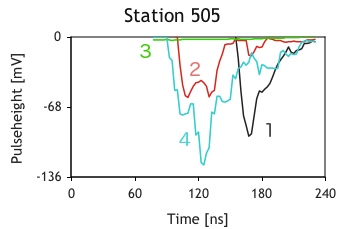
\includegraphics[scale=0.65]{Traces505}
    \caption{Ingewikkelde pulsvormen}
    \label{fig:Ingewikkelde-pulsvormen}
\end{figure}


\bigskip{}

In \figref{fig:Ingewikkelde-pulsvormen} valt het op dat de pulshoogte
van detector 2 (rood) kleiner is dan detector 1 (zwart).

\begin{minipage}[t]{1\columnwidth}%

\paragraph{Opdracht 4:}

Leg met de pulsintegraal (het pulsoppervlak) uit waarom er
waarschijnlijk evenveel deeltjes door detector 1 als door detector
2 zijn gegaan.

\begin{center}
    \rule{\textwidth}{0.3mm}\\
    \rule{\textwidth}{0.3mm}\\
    \rule{\textwidth}{0.3mm}\\
    \rule{\textwidth}{0.3mm}\\
\end{center}
\end{minipage}

\bigskip{}


In \figref{fig:Ingewikkelde-pulsvormen} valt het verder op dat detector
3 (groen) bijna geen puls geeft.

\begin{minipage}[t]{1\columnwidth}%

\paragraph{Opdracht 5:}

Verklaar waarom er binnen een station soms detectoren zijn
die een aantal deeltjes meten terwijl ander detectoren (bijna) niets
meten.

\begin{center}
    \rule{\textwidth}{0.3mm}\\
    \rule{\textwidth}{0.3mm}\\
    \rule{\textwidth}{0.3mm}\\
    \rule{\textwidth}{0.3mm}\\
\end{center}
\end{minipage}
\end{document}
